\فصل{مورد مطالعاتی: برنامه‌ی خرید برخط}

در این فصل روش ارائه‌شده در قسمت \رجوع{قسمت:چارچوب کلی} را بر روی نمونه‌ا‌ی اجرا خواهیم کرد، در ابتدا نمونه‌ را تشریح می‌کنیم و سپس مرحله به مرحله بر روی آن روش خود را اجرا می‌کنیم. در طول این قسمت ممکن است بر روی مورد مطالعاتی تغییراتی اعمال شود تا کارایی تحلیل‌ها یا روش آزمون ارائه‌شده بیشتر مشخص شود.  \newline\newline
\مهم{تشریح مورد مطالعاتی}

 نمونه‌ای که گفته ‌خواهد شد، یک برنامه‌ی خرید به صورت برخط است که از میکروسرویس‌های مستقل برای ارائه‌ی خدمت خود تشکیل شده‌ است. این میکروسرویس‌ها شامل میکروسرویس ورود با استفاده از گوگل\زیرنویس{Google}، ورود با استفاده از توئیتر\زیرنویس{Twitter} ورود با استفاده از لینکدین\زیرنویس{Linkedin}، سرویس خرید (انتخاب موارد خرید)، پرداخت با کارت اعتباری، پرداخت با پی‌پل\زیرنویس{PayPal} و تایید پرداخت است. می‌توان گفت که این خدمت با همکاری چند میکروسرویس ریزدانه‌تر محقق می‌شود؛ در این برنامه با آغاز روند خرید و اولین درخواست کاربر، اگر برنامه تشخیص بدهد که  نیاز به بررسی امنیتی درخواست کاربر وجود دارد میکروسرویس بررسی‌کننده‌ی امنیت این وظیفه را انجام می‌دهد و اگر درخواست را غیر مجاز یا خرابکارانه تشخیص دهد، بلافاصله فرآیند برنامه به اتمام می‌رسد و کاربر مجبور است درخواست دیگری برای آغاز خرید ارسال کند؛ اما در صورتی که درخواست از جنبه‌ی امنیتی تایید شود، کاربر باید احراز هویت خود را انجام دهد و این هدف توسط یکی از سه میکروسرویس ورود با استفاده از گوگل، ورود با استفاده از توئیتر ورود با استفاده از لینکدین به انتخاب کاربر، محقق می‌شود. اگر برنامه، بررسی امنیتی درخواست کاربر را لازم نداند، احراز هویت کاربر بلافاصله پس از درخواست کاربر صورت می‌پذیرد و اگر احراز هویت کاربر به درستی صورت نگیرد کاربر به حالت ابتدایی خود پس از درخواست شروع برنامه منتقل می‌شود و روند گفته‌‌شده در تلاش بعدی کاربر تکرار می‌شود؛ در غیر این صورت پس از احراز هویت کاربر، انتخاب کالاها و پر کردن سبد خرید توسط میکروسرویس نمایش و انتخاب کالاها، در تعامل با کاربر انجام می‌شود. 
 
 قطعه‌ی کدی که در پیوست ۱ آمده، ترجمه‌ی نمونه‌‌ای است که در شکل~\رجوع{شکل:مدل گردش کاری برنامه‌ی خرید برخط در یاول} آمده است.

پس از انتخاب کالاها، کاربر باید برای تکمیل خرید خود سبد خود را تسویه حساب کند، این وظیفه نیز توسط یکی از دو میکروسرویس پرداخت یعنی پرداخت با کارت اعتباری یا پرداخت با پی‌پل انجام می‌شود. اگر پرداخت موفقیت‌آمیز باشد جریان کنترل برنامه به میکروسرویس انتخاب کالا باز گردانده ‌ می‌شود و اگر پرداخت موفق باشد نیز میکروسرویس اتمام خرید که نحوه‌ی دریافت و تاییدیه‌ی پرداخت کاربر را به او نمایش می‌دهد خدمت خرید را به اتمام می‌رساند.

شکل~\رجوع{شکل: گردش کاری یک برنامه‌ی نمونه برای خرید برخط} نشان‌دهنده‌ی گردش کاری این برنامه است و شکل ~\رجوع{شکل:مدل گردش کاری برنامه‌ی خرید برخط در یاول} مدل‌سازی از برنامه‌ی پرداخت، به زبان یاول است.
\شروع{شکل}[t]
\centerimg{shopping-example-workflow}{14cm}
\vspace{0.5em}
\شرح{گردش کاری یک برنامه‌ی نمونه برای خرید برخط}
\برچسب{شکل: گردش کاری یک برنامه‌ی نمونه برای خرید برخط}
\پایان{شکل}


\شروع{شکل}[b]
\centerimg{shopping-example-yawl}{14cm}
\vspace{0.5em}
\شرح{مدل گردش کاری برنامه‌ی خرید برخط در یاول}
\برچسب{شکل:مدل گردش کاری برنامه‌ی خرید برخط در یاول}
\پایان{شکل}

در این مثال وظیفه‌ی "بررسی‌کننده‌ی امنیتی" انشعاب از نوع "یا" دارد و بعد از اتمام این وظیفه با توجه به پاسخ آن یا "شروع فرآیند ورود" بلافاصله آغاز می‌شود و یا این که بررسی‌کننده‌ی امنیتی خدمت برنامه، را منع می‌کند. همچنین وظیفه‌ی "شروع فرآیند ورود" دارای انشعاب از نوع "یای انحصاری" است زیرا کاربر تنها با یک روش از روش‌های سه‌گانه‌ی ورود ممکن (یعنی "ورود با گوگل"، "ورود با لینکدین" و "ورود با توئیتر")، می‌تواند احراز هویتش را انجام دهد و وارد حساب کاربری خود شود. اگر که پاسخ میکروسرویس‌هایی که عمل احراز هویت را انجام می‌دهند تایید هویت کاربر باشد، ورود کاربر موفقیت آمیز است و جریان کنترل برنامه به میکروسرویس "خرید (انتخاب موارد)" می‌رسد و در غیر این صورت جریان کنترل به ابتدای برنامه، یعنی "شروع خرید" باز می‌گردد.

پس از انتخاب موارد خرید توسط میکروسرویس "خرید"، بسته به انتخاب کاربر، یکی از میکروسرویس‌های پرداخت ("پرداخت با کارت اعتباری" و "پرداخت با پی‌پل") شروع به کار می‌کنند در نتیجه انشعاب در وظیفه‌ی "شروع پرداخت" از نوع "یای انحصاری" است. اگر پاسخ میکروسرویس‌ پرداخت، پرداخت موفقیت آمیز باشد، روند خرید تکمیل می‌شود و خدمت برنامه به پایان می‌رسد؛ اما اگر "پرداخت" ناموفق باشد، جریان کنترل به وظیفه‌ی "شروع پرداخت" بازگردانده می‌شود که در حین آن وظیفه کاربر مجددا به انتخاب سرویس پرداخت می‌پردازد. با توجه به عملکرد مورد انتظار از برنامه و شرایط گفته‌شده، وظیفه‌ی "شروع پرداخت" پیوند از نوع "یای انحصاری" دارد. \newline\newline


\مهم{تحلیل بررسی پیوند از نوع ``یا'' در حلقه}

در برنامه‌ی خرید برخط، سناریویی را در نظر بگیرید که طراح برای شروع کار میکروسرویس "شروع خرید"، شرط انجام کار در میکروسرویس "احراز هویت و ورود" قبلی را لحاظ می‌کند و گردش کار مشخص شده در شکل ~\رجوع{شکل:وجود پیوند از نوع ``یا'' در مدل برنامه‌ی خرید برخط در یاول} را تعریف می‌کند. 
\شروع{شکل}[t]
\centerimg{no-or-join-in-loop-yawl}{14cm}
\vspace{0.5em}
\شرح{وجود پیوند از نوع ``یا'' در مدل}
\برچسب{شکل:وجود پیوند از نوع ``یا'' در مدل برنامه‌ی خرید برخط در یاول}
\پایان{شکل}
در این گردش کاری وظیفه‌ی "شروع خرید" که دارای پیوند از نوع "یا" است در انتظار مشخص شدن وضعیت جریان‌های ورودی‌ خود است تا پس از آن کار خود را آغاز کند، در حالی که مشخص شدن وضعیت ورودی‌های آن به فعال بودن با نبودن خروجی وظیفه‌ی "احراز هویت و ورود" بستگی دارد؛ در حالی که مشخص شدن فعال یا غیر فعال بودن خروجی این وظیفه به مشخص بودن وضعیت "آغاز خرید" بستگی دارد؛ در نتیجه گردش کار در وضعیت بن‌بست قرار گرفته است که وضعیتی نامطلوب است و دلیل آن نیز قرار گرفتن وظیفه‌ای با پیوند از وضعیت "یا" در حلقه است.

اظهار تولید شده برای گردش کاری در شکل ~\رجوع{شکل:وجود پیوند از نوع ``یا'' در مدل برنامه‌ی خرید برخط در یاول}، در زیر آمده است.



\شروع{شکل}[H]
\raggedright
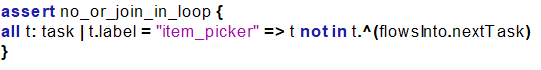
\includegraphics[width=10cm]{or-join-in-loop-shopping}
\vspace{0.5em}
\برچسب{شکل: اظهار تولیدشده برای اطمینان از عدم وجود پیوند از نوع ``یا'' در حلقه در برنامه‌‌ی خرید برخط}
\پایان{شکل}



\مهم{تحلیل بررسی قابل دستیابی بودن میکروسرویس‌ها}

در مثال برنامه‌ی خرید برخط، فرض کنید که طراح در میکروسرویس "تاییدکننده‌ی پرداخت" شرط فعال شدن میکروسرویس "اتمام خرید" را این‌گونه تعریف کند:


\شروع{شکل}[H]
\raggedright
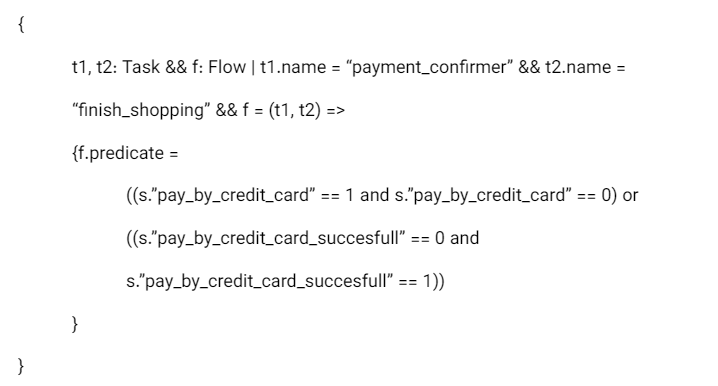
\includegraphics[width=10cm]{corrupted-condition-results-inreachablility}
\vspace{0.5em}
\برچسب{شکل: شرط نادرست در جریان خروجی که سبب غیر قابل دسترس بودن وظیفه می‌شود}
\پایان{شکل}

در حالی که مقدار شرط صحیح این‌گونه است:



\شروع{شکل}[H]
\raggedright
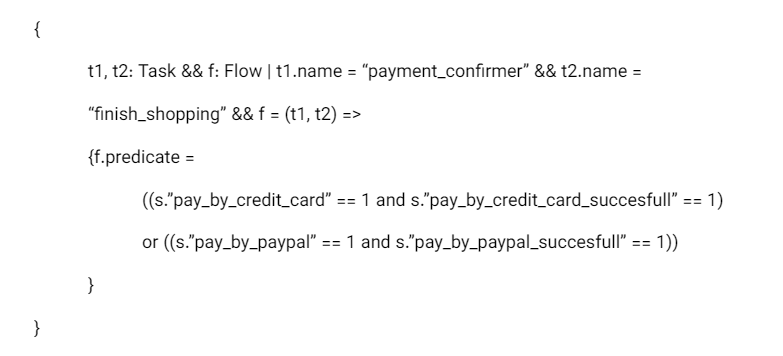
\includegraphics[width=10cm]{right-condition-in-output-flow}
\vspace{0.5em}
\برچسب{شکل: شرط درست در جریان خروجی}
\پایان{شکل}



در این صورت هرگز ارزش مسند 
\شروع{شکل}[H]
\raggedright
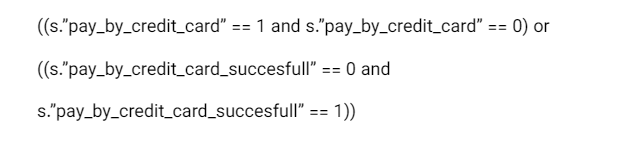
\includegraphics[width=10cm]{corrupted-predicate}
\vspace{0.5em}
\برچسب{شکل: نمونه مسند اشتباه در جریان خروجی }
\پایان{شکل}
برابر "درست" نخواهد شد. در نتیجه هیچ گاه به وظیفه‌ی "اتمام خرید" در زمان اجرای گردش کار نخواهیم رسید و در حقیقت وظیفه‌ی "اتمام خرید" در گردش کاری طراحی شده غیرقابل دسترسی است. اظهار افزوده شده برای یافتن مثال نقض این گزاره به صورت زیر به توصیف گردش کار افزوده می‌شود. \newline\newline



\شروع{شکل}[H]
\raggedright
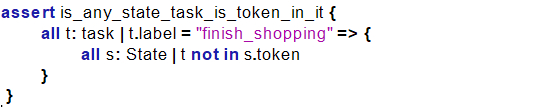
\includegraphics[width=10cm]{reachability-assertion-shopping}
\vspace{0.5em}
\برچسب{شکل: اظهار نوشته‌شده برای قابل دسترس بودن در نمونه‌ی خرید}
\پایان{شکل}
 

 \مهم{تحلیل بررسی منتظر ماندن دو پیوند از نوع ``یا'' برای یکدیگر}
 \شروع{شکل}[t]
\raggedright
\centerimg{two-pending-or-joins}{12cm}
\vspace{0.5em}
\شرح{منتظر بودن دو پیوند از نوع ``یا'' در مثال خرید برخط}
\برچسب{شکل: منتظر بودن دو پیوند از نوع ``یا'' در مثال خرید برخط}
\پایان{شکل}
 مجددا برنامه‌ی خرید برخط را در نظر بگیرید فرض کنید در این نمونه طراح برای نمایش اجرای دو بار "خرید" به صورت پشت سر هم، توسط کاربر گردش کار زیر را طراحی می‌کند، در این گردش کار، میکروسرویس "آغاز خرید"، دارای پیوند از نوع "یا" است و برای آغاز به کار در انتظار مشخص شدن وضعیت جریان‌های ورودی خود است.در حالی که یکی از ورودی‌های آن میکروسرویس "احراز هویت و ورود" است که خود دارای پیوند از نوع "یا" است و مشخص شدن وضعیت ورودی‌های آن به مشخص شدن وضعیت وظیفه‌ی "آغاز خرید"، بستگی دارد. در نتیجه گردش کار دچار بن‌بست می‌شود که وضعیتی نامطلوب است.


برای پیدا کردن این وضعیت در گردش کار اظهار زیر را به توصیف کلی اضافه می‌کنیم: \newline\newline



\شروع{شکل}[H]
\raggedright
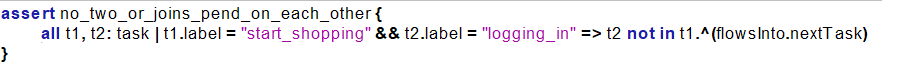
\includegraphics[width=16cm]{two-pending-or-joins-assertion-in-shopping}
\vspace{0.5em}
\برچسب{شکل: اظهار نوشته‌شده برای بررسی منتظر بودن دو پیوند از نوع ``یا'' در مثال خرید برخط}
\پایان{شکل}


\مهم{تولید موارد آزمون}

در روشی که گفته شد برای تولید موارد آزمون، از مسندهای شرطی در انشعاب‌ها استفاده می‌کنیم، اکنون برای مورد مطالعاتی‌، یعنی برنامه‌ی خرید برخط، به تولید موارد آزمون می‌پردازیم.

همان‌طور که در شکل زیر می‌بینید خروج از "تاییدکننده‌ی پرداخت" و ورود به "اتمام خرید" شرط زیر را داراست:
\شروع{شکل}[t]
\centerimg{payment-test-example.png}{8cm}
\vspace{0.5em}
\شرح{میکروسرویس تایید پرداخت دارای گزاره‌های شرطی برای ایجاد آزمون\newline\newline}
\برچسب{میکروسرویس تایید پرداخت دارای گزاره‌های شرطی برای ایجاد آزمون}
\پایان{شکل}


\شروع{شکل}[H]
\raggedright
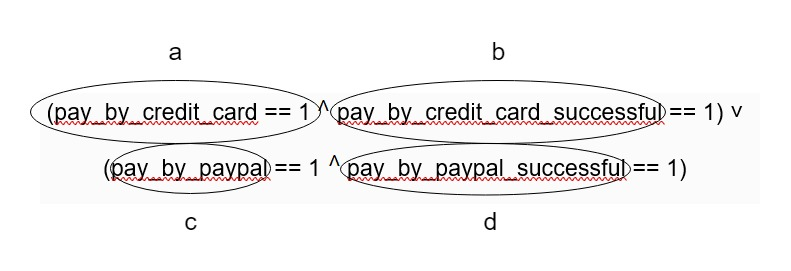
\includegraphics[width=10cm]{shopping-clauses}
\vspace{0.5em}
\برچسب{شکل: گزاره‌های موجود در جریان‌های خروجی وظیفه‌ی پرداخت}
\پایان{شکل}
برای تولید موارد آزمون بر اساس معیار پوشش گزاره‌ی فعال محدود، درخت گزاره‌های این مسند را تشکیل می‌دهیم و آن را حل میکنیم و سپس زوج موارد آزمون را از طبق جدول صحت گزاره‌ها استخراج می‌کنیم.
\شروع{شکل}[H]
\raggedright
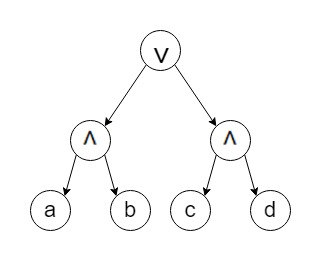
\includegraphics[width=5cm]{shopping-expression-tree}
\vspace{0.5em}
\برچسب{شکل: درخت عبارت وظیفه‌ی پرداخت در برنامه‌ی خرید برخط}
\پایان{شکل}
\شروع{شکل}[H]
\raggedright
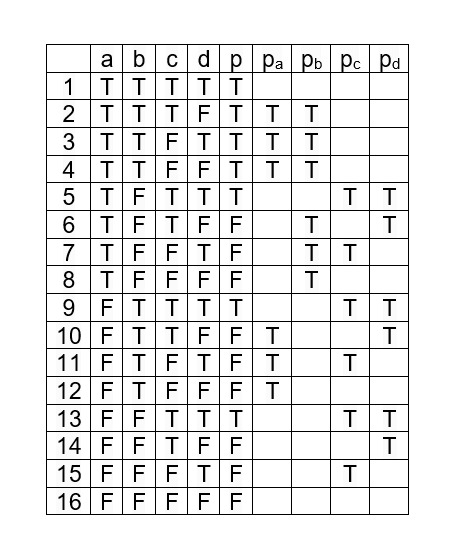
\includegraphics[width=10cm]{shoppping-payment-racc}
\vspace{0.5em}
\برچسب{شکل: درخت عبارت وظیفه‌ی پرداخت در برنامه‌ی خرید برخط}
\پایان{شکل}

طبق جدول صحتی که در بالا آمده است زوج‌ موارد آزمون برای هر کدام از گزاره‌های
$\set{a, b, c, d}$
به صورت زیر به دست می‌آید:

\شروع{فقرات}
\فقره برای a : 
$\set{(2, 10), (3, 11), (4, 12)}$
\فقره برای b : 
$\set{(2, 6), (3, 7), (4, 8)}$
\فقره برای c : 
$\set{(5, 7), (9, 11), (13, 15)}$
\فقره برای d : 
$\set{(5, 6), (9, 10), (13, 14)}$
\پایان{فقرات}

برای نمونه دو توصیفی که برای اجرای زوج موارد آزمون (۲و ۶) برای گزاره‌ی b ایجاد می‌شود به صورت زیر است:



\شروع{شکل}[H]
\raggedright
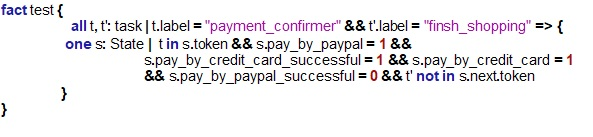
\includegraphics[width=16cm]{example-test-specification-b-equals-true}
\vspace{0.5em}
\برچسب{شکل: گزاره‌های موجود در جریان‌های خروجی وظیفه‌ی پرداخت گزاره‌ی ۲}
\پایان{شکل}

\شروع{شکل}[H]
\raggedright
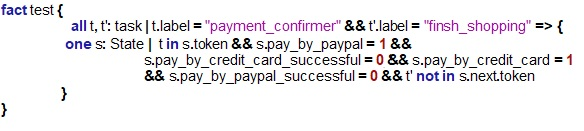
\includegraphics[width=16cm]{example-test-specification-b-equals-false}
\vspace{0.5em}
\برچسب{شکل: گزاره‌های موجود در جریان‌های خروجی وظیفه‌ی پرداخت ۶}
\پایان{شکل}



پس از تایید امنیتی (در صورت نیاز)، کاربر می‌تواند روش ورود خود را بر اساس سلیقه‌ی خود انتخاب کند. برای این منظور 3 متغیر برای کاربر در نظر گرفته شده‌ است و او می‌تواند فقط یکی از آن‌ها را انتخاب کند و بسته به متغیر انتخاب شده‌ یکی از میکروسرویس‌های ورود شروع به کار می‌کنند و هویت کاربر را احراز می‌کنند. برای مثال، خروج از "شروع فرآیند ورود" و ورود به روش‌ "ورود با گوگل'' شرط زیر را داراست:
\شروع{شکل}[b]
\centerimg{example2}{8cm}
\vspace{0.5em}
\شرح{شروع فرآیند ورود دارای گزاره‌های شرطی برای ایجاد آزمون\newline\newline}
\برچسب{شروع فرآیند ورود دارای گزاره‌های شرطی برای ایجاد آزمون}
\پایان{شکل}


\شروع{شکل}[H]
\raggedright
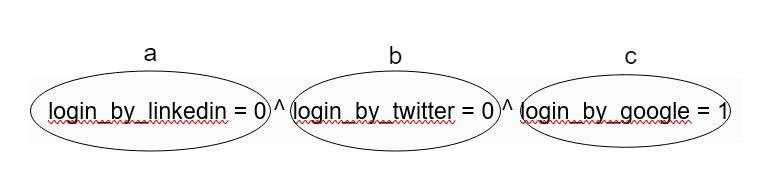
\includegraphics[width=10cm]{login-clauses}
\vspace{0.5em}
\برچسب{شکل: گزاره‌های موجود در جریان‌های خروجی وظیفه‌ی ورود}
\پایان{شکل}
برای این مسند هم، درخت گزاره‌ها را تشکیل می‌دهیم و آن را حل میکنیم و سپس زوج موارد آزمون را از طبق جدول صحت گزاره‌ها استخراج می‌کنیم.
\شروع{شکل}[H]
\raggedright
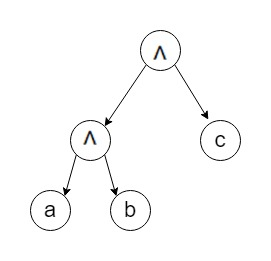
\includegraphics[width=5cm]{login-expression-tree}
\vspace{0.5em}
\برچسب{شکل: درخت عبارت وظیفه‌ی ورود در برنامه‌ی خرید برخط}
\پایان{شکل}
\شروع{شکل}[H]
\raggedright
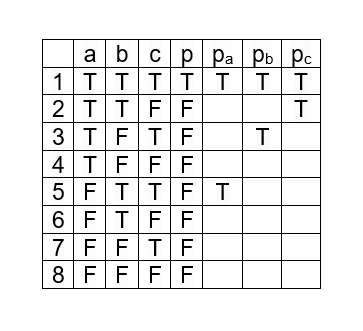
\includegraphics[width=10cm]{shoppping-login-racc}
\vspace{0.5em}
\برچسب{شکل: جدول صحت وظیفه‌ی ورود در برنامه‌ی خرید برخط}
\پایان{شکل}

طبق جدول صحتی که در بالا آمده است زوج‌ موارد آزمون برای هر کدام از گزاره‌های
$\set{a, b, c}$
به صورت زیر به دست می‌آید:

\شروع{فقرات}
\فقره برای a: 
$\set{(1, 5)}$
\فقره برای b: 
$\set{(1, 3)}$
\فقره برای c: 
$\set{(1, 2)}$
\پایان{فقرات}

برای نمونه دو توصیفی که برای اجرای زوج موارد آزمون (۱ و ۵) برای گزاره‌ی a ایجاد می‌شود به صورت زیر است:



\شروع{شکل}[H]
\raggedright
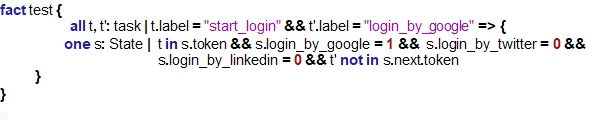
\includegraphics[width=16cm]{login-test-specification-a-equals-true}
\vspace{0.5em}
\برچسب{شکل: گزاره‌های موجود در جریان‌های خروجی وظیفه‌ی پرداخت گزاره‌ی ۱}
\پایان{شکل}

\شروع{شکل}[H]
\raggedright
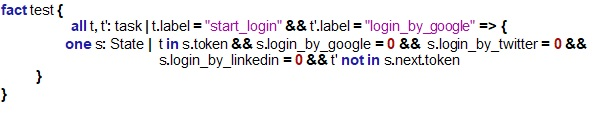
\includegraphics[width=16cm]{login-test-specification-a-equals-false}
\vspace{0.5em}
\برچسب{شکل: گزاره‌های موجود در جریان‌های خروجی وظیفه‌ی پرداخت ۵}
\پایان{شکل}

  
